\chapter{Pile-up}
\label{chap:pileup}

\section{Scope and principal conclusion}
\label{sec:pileup_scope}

The pile-up studies ask a narrower question than a generic waveform-classifier
benchmark: how much of the high-current pulse population is consistent with
overlapping beam particles, what effective live-time should enter the rate
model, and whether learned waveform methods should replace the transparent
topology and template analyses.  The data contain no direct truth label for a
real pile-up pulse.  The analysis therefore separates three evidential layers:
first, current-dependent topology rates measured directly in the beam data;
second, raw-waveform live-time measurements that revise the effective time
window used in the Poisson occupancy calculation; and third, injected
two-pulse closure tests that rank reconstruction algorithms under a controlled
but synthetic truth definition.

The main physics conclusion is that the originally quoted maximum rate is
reproducible only as an assumption.  The S10 reproduction gives
$R_{\max}=4.222$ MHz when $\tau_{\mathrm{eff}}=90$ ns is inserted by hand.
However, the directly measured waveform live-time is materially longer:
the run-held-out template measurement gives a 10\% live-time of
$124.79$ ns with a 95\% bootstrap confidence interval
$[123.32,126.33]$ ns.  Rescaling the same occupancy limit with this
measured window gives
\begin{equation}
  R_{\max}^{\mathrm{meas}}
  =
  \frac{\mu_{\max}}{\tau_{\mathrm{live}}}
  =
  \frac{0.380}{124.79\ \mathrm{ns}}
  =
  3.05\ \mathrm{MHz},
  \label{eq:pileup_rmax_revision}
\end{equation}
not 4.22 MHz.  This is the central pile-up revision.

The method winner depends on the estimand.  For the beam-rate claim, the
winner is the traditional topology plus Poisson/live-time analysis: it is
transparent, directly tied to current and topology, and does not require a
synthetic label.  For template-like injected two-pulse decomposition, compact
neural methods, especially the MLP and the 18-sample one-dimensional CNN,
achieve lower timing RMS than the bounded two-pulse template fit.  That neural
advantage is not adopted as the beam-rate estimator because it comes with a
higher failure rate and because injected overlap truth is not real
high-current truth.

\section{Rate model and live-time definition}
\label{sec:pileup_rate_model}

The conventional occupancy calculation models the number of unresolved
particles in an effective live-time window as Poisson distributed.  If
$\mu=R\tau_{\mathrm{eff}}$ is the expected number of particles in the window,
then the no-more-than-one-particle probability is
\begin{equation}
  P(N \leq 1) = e^{-\mu}(1+\mu),
  \label{eq:pileup_poisson}
\end{equation}
and an allowed occupancy $\mu_{\max}$ maps to a maximum rate
\begin{equation}
  R_{\max} = \frac{\mu_{\max}}{\tau_{\mathrm{eff}}}.
  \label{eq:pileup_rmax}
\end{equation}
S10 reproduced the documented combined requirement $|dt|<1$ ns and
area $<20\%$ with $\mu_{\max}=0.380$.  With the historical
$\tau_{\mathrm{eff}}=90$ ns, this gives
$R_{\max}=4.222$ MHz.  The reproduction gate also recovered all six
low-current and high-current topology fractions within the predeclared
tolerance, so the discrepancy is not in event counting; it is in the
interpretation of the time window.

The S10b and S10c studies estimated the live-time directly from raw B-stack
waveforms.  For each held-out run, selected pulses were pedestal subtracted,
timed with CFD20, aligned by stave, and median combined.  The post-peak tail
was fit with
\begin{equation}
  y(t) = c + a \exp(-t/\tau),
  \label{eq:pileup_tail_fit}
\end{equation}
and the live-time was defined as the crossing below a chosen fraction of the
pulse amplitude.  A run-held-out ridge regressor from pulse-shape summaries to
the same live-time target was used as the ML comparison.  It excluded run,
event number, current labels, and direct last-above-threshold width features.

\begin{table}[H]
\centering
\caption{Measured waveform live-time and the implied rate revision.  Intervals
are 95\% bootstrap confidence intervals over held-out runs.  The traditional
method is the median-template exponential crossing; the ML method is the
run-held-out ridge live-time predictor.}
\label{tab:pileup_livetime}
\resizebox{\textwidth}{!}{%
\begin{tabular}{lrrrr}
\toprule
Threshold & Template live-time (ns) & Ridge live-time (ns) & $R_{\max}$ (MHz) & Above 90 ns? \\
\midrule
5\% & 141.06 [139.29, 143.01] & 124.75 [122.59, 126.69] & 2.69 & yes \\
10\% & 124.79 [123.32, 126.33] & 123.22 [120.71, 125.61] & 3.05 & yes \\
20\% & 101.87 [100.90, 102.83] & 119.18 [115.60, 122.48] & 3.73 & yes \\
Noise floor & 161.18 [158.76, 163.61] & 120.30 [117.03, 123.22] & 2.36 & yes \\
\bottomrule
\end{tabular}
}
\end{table}

The threshold scan is important because it tests whether the 90 ns value could
be recovered by a reasonable alternative crossing definition.  It could not:
even the shortest traditional crossing, the 20\% threshold, has its lower
bootstrap bound above 100 ns.  The ridge predictor broadly agrees with the
10\% result but is not the primary rate estimator, since the template crossing
is simpler and closer to the physical definition of an unresolved pulse tail.

\begin{figure}[H]
\centering
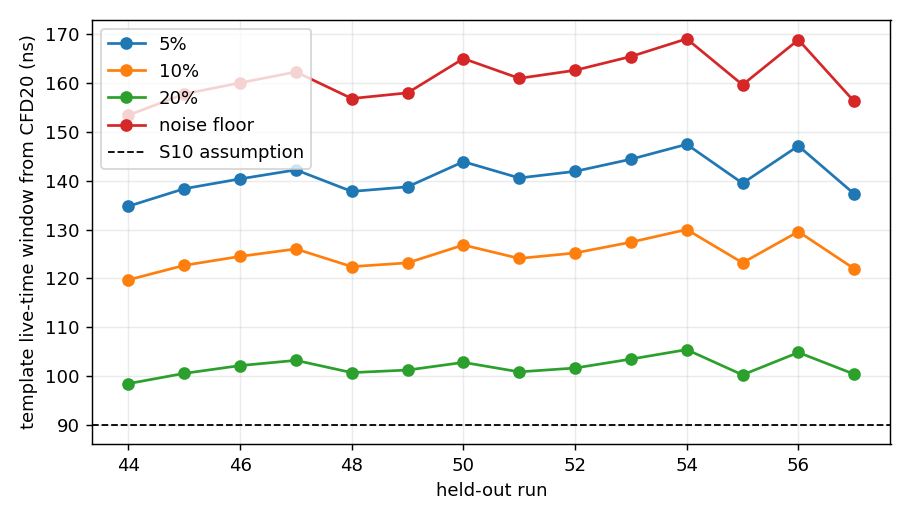
\includegraphics[width=0.92\textwidth]{../figures/reports/1781007337.1308.7dc86005/fig_threshold_scan_by_run.png}
\caption{Run-held-out live-time threshold scan from S10c.  All scanned
template definitions remain above the historical 90 ns assumption.}
\label{fig:pileup_threshold_scan}
\end{figure}

\section{Current-dependent topology excess}
\label{sec:pileup_current_topology}

The beam-current comparison uses selected B-stave events as the denominator.
Runs 46 and 47 form the 2 nA reference, while runs 44, 45, and 48--57 form the
20 nA sample.  The most interpretable traditional observable is the downstream
topology fraction per selected event.  S10 measured a rise from 2.312\% at
2 nA to 3.341\% at 20 nA, a high-minus-low excess of 1.029 percentage points
with a 95\% binomial confidence interval of [0.637, 1.421] percentage points.
Equivalently, about 30.8\% of the high-current downstream rate is attributable
to the current-dependent excess under this topology definition.

\begin{table}[H]
\centering
\caption{S10 current-topology reproduction.  Fractions are per selected event
and reproduce the documented values within the predeclared 0.0015 tolerance.}
\label{tab:pileup_topology}
\begin{tabular}{lrrr}
\toprule
Observable & 2 nA & 20 nA & High/low ratio \\
\midrule
Multi-stave fraction & 0.015588 & 0.026806 & 1.720 \\
$\geq 3$-stave fraction & 0.004111 & 0.008538 & 2.077 \\
Downstream fraction & 0.023124 & 0.033414 & 1.445 \\
\bottomrule
\end{tabular}
\end{table}

The corresponding ML diagnostic in S10 was an injection-trained logistic
pile-up score using waveform-shape features such as area-to-peak ratio, tail
fractions, late fractions, early fractions, width handles, and post-peak
structure.  It was trained on synthetic clean versus injected two-pulse
waveforms, not on real beam pile-up truth.  On real selected pulses the
low-current-trained score mean rose from 0.1213 to 0.1574, a high/low ratio of
1.297.  This confirms that waveform morphology changes with current, but the
ratio is much smaller than the beam-current ratio and remains a proxy rather
than a calibrated pile-up probability.

\begin{figure}[H]
\centering
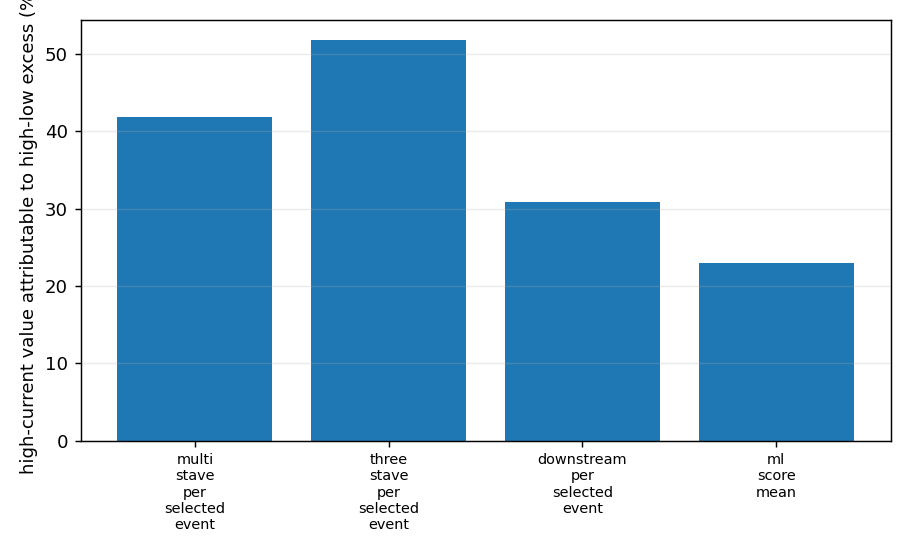
\includegraphics[width=0.86\textwidth]{../figures/reports/1780997954.15277.548b01a3__s10_pileup_rate_model/fig_current_excess.png}
\caption{S10 current-dependent excess.  The topology observable gives the
physics-facing current-rate handle; waveform ML scores are used as diagnostics
of morphology rather than direct rate estimators.}
\label{fig:pileup_current_excess}
\end{figure}

\section{Two-pulse reconstruction benchmark}
\label{sec:pileup_two_pulse}

The two-pulse studies provide controlled algorithm rankings under a synthetic
truth definition.  The construction uses S01-style empirical B-stack templates
and real single-pulse residuals from raw selected pulses.  Training uses runs
58--62 and evaluation holds out runs 63 and 65.  The traditional reconstruction
is a bounded two-pulse template fit: it initializes with CFD20, scans first
pulse timing offsets and fixed separation hypotheses, solves amplitudes and
baseline by least squares, and records constrained-fit failures.  The neural
comparators are compact waveform models trained on the same injected mixtures:
an MLP classifier/regressor for overlap probability, two times, and two
amplitudes, and a compact 18-sample one-dimensional CNN with convolutional
feature extraction and the same decomposition heads.

For a waveform $x(t)$, the traditional model is
\begin{equation}
  x(t) = b + A_1 T(t-t_1) + A_2 T(t-t_2) + \epsilon(t),
  \label{eq:pileup_two_pulse_template}
\end{equation}
with a template $T$ built only from training runs.  The fit minimizes the
sum of squared residuals over the scanned hypotheses.  The neural models
replace the explicit hypothesis scan with learned functions
$f_{\theta}(x)=(\hat p,\hat t_1,\hat t_2,\hat A_1,\hat A_2)$, optimized on
injected mixtures from the training runs.

\begin{table}[H]
\centering
\caption{Injected two-pulse reconstruction benchmark.  Intervals are 95\%
bootstrap intervals over held-out run blocks.  The neural methods win on time
RMS and AP, while the traditional fit wins on failure rate.}
\label{tab:pileup_two_pulse}
\resizebox{\textwidth}{!}{%
\begin{tabular}{lrrrr}
\toprule
Method & AP & Time RMS (ns) & Charge res68 & Failure rate \\
\midrule
Bounded two-pulse template fit & 0.767 [0.737, 0.796] & 13.30 [12.00, 14.56] & 0.098 [0.089, 0.109] & 0.168 [0.139, 0.200] \\
Compact MLP & 0.851 [0.820, 0.879] & 10.67 [9.62, 11.84] & 0.078 [0.068, 0.084] & 0.295 [0.261, 0.331] \\
Compact 18-sample CNN & 0.868 [0.864, 0.874] & 10.01 [9.88, 10.14] & 0.080 [0.075, 0.085] & 0.228 [0.220, 0.237] \\
\bottomrule
\end{tabular}
}
\end{table}

S10d also translated the recovery benchmark into a resolvability live-time:
the first tested separation after which all larger separations satisfy
\begin{equation}
  |\mathrm{median\ timing\ bias}| < 1\ \mathrm{ns},
  \qquad
  |\mathrm{median\ total\ area\ bias}| < 0.20 .
  \label{eq:pileup_resolvability_criteria}
\end{equation}
Under this definition, the
bounded template fit becomes resolvable at 60 ns with bootstrap interval
[40, 60] ns, while the compact MLP reaches 20 ns with interval [15, 60] ns.
The point estimate favors ML, but the upper confidence limit overlaps the
template fit and the MLP failure rate is almost twice as large.

\begin{figure}[H]
\centering
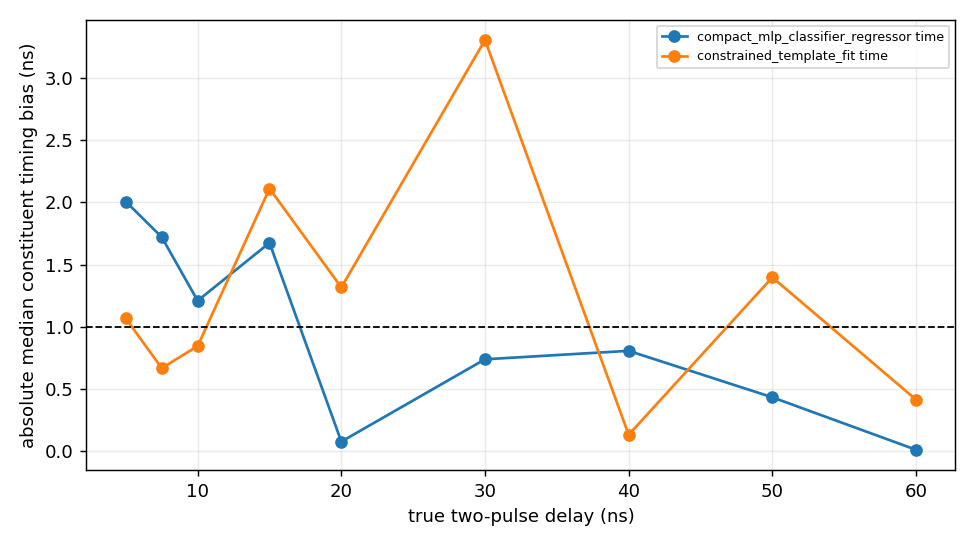
\includegraphics[width=0.88\textwidth]{../figures/reports/1781007337.1325.2241031c/fig_resolvability_delay_bias.png}
\caption{S10d resolvability-delay bias curves for the bounded template fit and
compact MLP.  Neural reconstruction reaches the bias criterion at a shorter
point estimate, but the operational interpretation is limited by failure rate
and synthetic injection truth.}
\label{fig:pileup_resolvability}
\end{figure}

\section{Failure-aware abstention}
\label{sec:pileup_abstention}

Average timing RMS is not sufficient for a production pile-up correction.  A
method that gives excellent estimates for many events but silently fails on a
large tail can bias downstream timing or charge analyses.  P05b therefore
calibrated abstention gates on the S11a injected benchmark.  Bad recovery was
defined as a base-method failure, constituent-time RMS above 12 ns, or absolute
charge bias above 0.20.  The traditional gate used train-run-only cuts on fit
failure, fractional SSE improvement, a $\chi^2/\mathrm{ndf}$ proxy, fitted
separation, and amplitude ratio.  The ML gate used an isotonic-calibrated
logistic risk model over normalized waveform features and fit diagnostics.

\begin{table}[H]
\centering
\caption{P05b failure-aware operating points.  The traditional gate is more
selective and safer among accepted events; the ML gate keeps more coverage but
accepts a higher bad-recovery rate.}
\label{tab:pileup_abstention}
\resizebox{\textwidth}{!}{%
\begin{tabular}{lrrrr}
\toprule
Gate & Coverage & Accepted RMS (ns) & Charge res68 & Bad recovery \\
\midrule
Traditional quality cuts & 0.343 & 7.42 [6.61, 8.26] & 0.070 [0.067, 0.075] & 0.092 [0.082, 0.104] \\
ML isotonic failure gate & 0.728 & 8.44 [8.28, 8.59] & 0.064 [0.064, 0.069] & 0.144 [0.131, 0.157] \\
\bottomrule
\end{tabular}
}
\end{table}

This result explains why the chapter does not promote the neural decomposers
as the pile-up correction by default.  The CNN and MLP are the timing-RMS
winners on injected overlaps, but the traditional quality gate provides a
lower-risk accepted sample.  The practical conclusion is an operating-point
trade-off: neural recovery is useful for diagnostic studies and perhaps for
high-coverage correction studies, while conservative template-quality cuts are
safer when a low bad-recovery rate is the controlling requirement.

\begin{figure}[H]
\centering
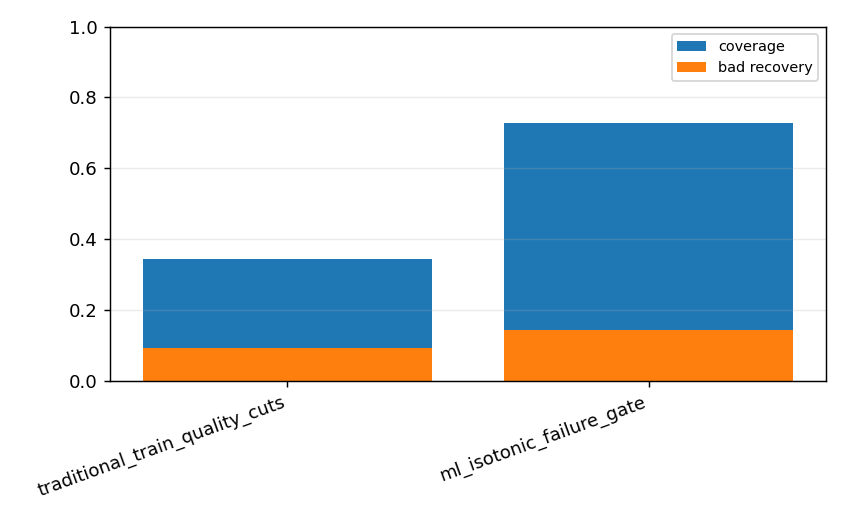
\includegraphics[width=0.82\textwidth]{../figures/reports/1781014241.437.0e0024cb/fig_gate_coverage_bad_rate.png}
\caption{P05b risk-coverage comparison for failure-aware two-pulse recovery.
The ML gate buys coverage; the traditional gate buys a cleaner accepted
sample.}
\label{fig:pileup_abstention}
\end{figure}

\section{CWoLa current-scaling diagnostic}
\label{sec:pileup_cwola}

S13b tested whether a weakly supervised current classifier could reproduce the
S10 waveform-score current scaling under independent run transfer.  The method
is Classification Without Labels: train a classifier to distinguish mixtures
of high-current and low-current selected pulses, then interpret the learned
score as a morphology-sensitive current discriminator rather than as a
per-pulse truth label.  The CWoLa model was a random forest trained on
normalized waveform samples plus pulse-shape summaries.  It excluded run,
event number, current labels as features, and downstream/topology labels.

The split was by run block.  The A-to-B fold trained on low run 46 plus high
runs 44, 45, and 48--51, then tested on low run 47 plus high runs 52--57.  The
B-to-A fold reversed the partition.  Bootstrap intervals resampled held-out
runs within current group; with only two low-current runs, the low-current
component is necessarily a limited systematic.

\begin{table}[H]
\centering
\caption{S13b current-scaling comparison.  CWoLa transfers as a modest
waveform-shape current discriminator, but the topology ratio remains the
stronger physics-facing rate handle.}
\label{tab:pileup_cwola}
\begin{tabular}{lrr}
\toprule
Method & High/low score or rate ratio & Held-out current AUC \\
\midrule
Single traditional shape feature & 1.064 [0.982, 1.095] & 0.633 [0.346, 0.748] \\
CWoLa random forest shape score & 1.220 [1.193, 1.257] & 0.668 [0.656, 0.682] \\
Shuffled-label random forest & 1.020 [1.012, 1.032] & 0.559 [0.538, 0.590] \\
Traditional downstream topology & 1.445 [1.220, 2.542] & -- \\
\bottomrule
\end{tabular}
\end{table}

\begin{figure}[H]
\centering
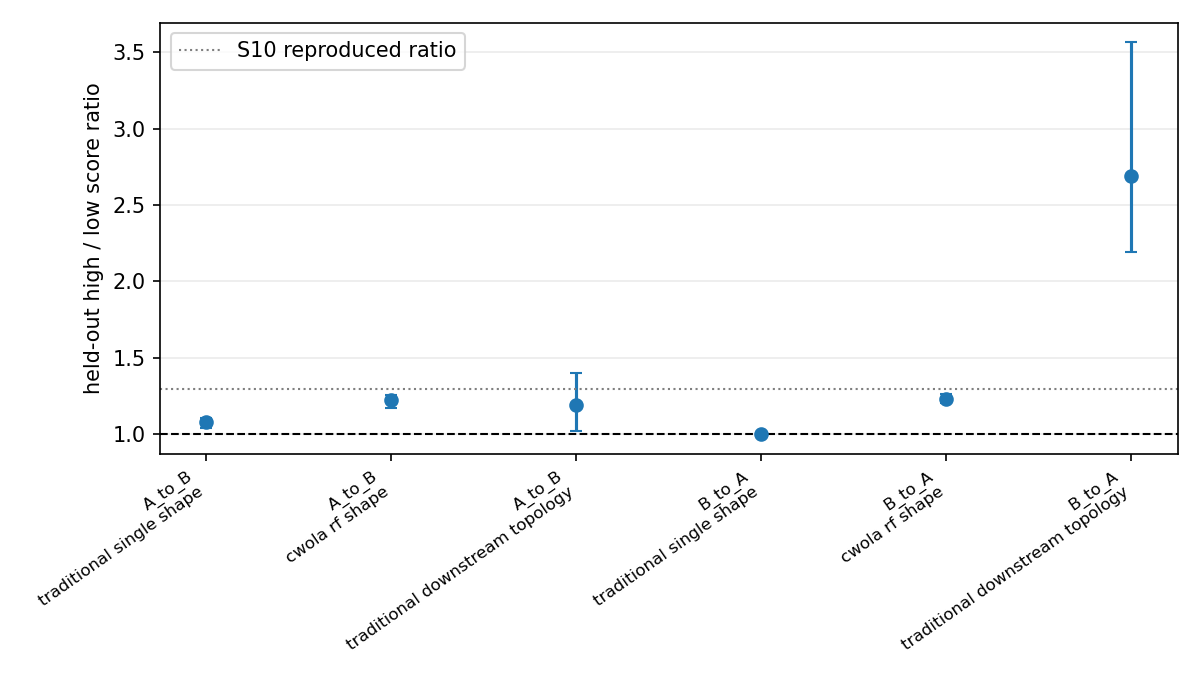
\includegraphics[width=0.86\textwidth]{../figures/reports/1781000867.546938.20f0173c/fig_run_block_score_ratios.png}
\caption{S13b run-block score ratios.  The CWoLa score transfers beyond the
S10 two-low-run reference, but its magnitude is smaller than the topology
ratio and should be interpreted diagnostically.}
\label{fig:pileup_cwola}
\end{figure}

\section{Systematics and caveats}
\label{sec:pileup_systematics}

The dominant systematic is the absence of real pile-up truth.  Current
dependence is directly measured, but individual pulses are not labeled as
single-particle or multi-particle beam events.  Therefore the topology excess
and Poisson/live-time calculation support a rate revision, whereas the MLP,
CNN, ridge, and CWoLa models support algorithmic or diagnostic statements.

The live-time systematic is definitional.  A 10\% threshold gives the
headline 3.05 MHz revision, but a 20\% threshold gives 3.73 MHz and a
noise-floor threshold gives 2.36 MHz.  All reasonable scanned definitions are
longer than 90 ns, so the qualitative revision is stable even though the exact
rate depends on the chosen crossing.  This uncertainty should be propagated as
a live-time-definition envelope rather than hidden inside a single nominal
number.

The injection systematic affects the two-pulse reconstruction winner.  The
injected mixtures use empirical templates and real residuals, but they are
still generated from the same template family used by the reconstruction
benchmark.  Real high-current pile-up can include saturation, baseline
excursions, broad-late pulse shapes, and topology effects that are not fully
represented.  Strict run splits, event-overlap checks, and shuffled-label
sentinels reduce leakage risk, but they cannot convert injected truth into
measured beam truth.

Finally, the high-current excess is heterogeneous.  Follow-up studies find
that after matching on amplitude, baseline, and topology the excess
concentrates in high-amplitude, large-baseline-lowering, broad-late pulses.
This heterogeneity is precisely why topology remains the rate handle and ML
scores remain monitors: a scalar waveform score can detect current-sensitive
morphology, but it does not by itself identify a clean Poisson pile-up
component.

\section{Chapter verdict}
\label{sec:pileup_verdict}

For the pile-up rate model, the traditional analysis wins.  The reproducible
occupancy equation gives 4.222 MHz only under the historical 90 ns assumption;
the measured waveform live-time revises the preferred 10\% estimate to
3.05 MHz, with a threshold-definition envelope spanning roughly
2.36--3.73 MHz in the S10c scan.  For injected two-pulse recovery, neural
methods win the timing-RMS benchmark: the compact MLP reaches 10.67 ns and the
18-sample CNN reaches 10.01 ns, compared with 13.30--13.90 ns for the bounded
template fit.  But the bounded fit and its train-derived quality cuts remain
the safer operational choice when bad-recovery rate is the controlling
criterion.  CWoLa random forests provide a useful current-scaling diagnostic
with a high/low ratio of 1.220 and held-out AUC of 0.668, but they do not
replace the downstream topology ratio of 1.445 as the physics-facing evidence.
